%%%% Proceedings format for most of ACM conferences (with the exceptions listed below) and all ICPS volumes.
\documentclass[sigconf, nonacm=true]{acmart}

% \settopmatter{printacmref=false} % Removes citation information below abstract
% \renewcommand\footnotetextcopyrightpermission[1]{} % removes footnote with conference information in first column
% \pagestyle{plain} % removes running headers

%
% defining the \BibTeX command - from Oren Patashnik's original BibTeX documentation.
\def\BibTeX{{\rm B\kern-.05em{\sc i\kern-.025em b}\kern-.08emT\kern-.1667em\lower.7ex\hbox{E}\kern-.125emX}}

\usepackage{array}
\newcolumntype{?}{!{\vrule width 2pt}}

\usepackage{caption}
\usepackage{subcaption}

\begin{document}

%
% The "title" command has an optional parameter, allowing the author to define a "short title" to be used in page headers.
\title{Methods for Efficient N-Gram Representation}

%
% The "author" command and its associated commands are used to define the authors and their affiliations.
% Of note is the shared affiliation of the first two authors, and the "authornote" and "authornotemark" commands
% used to denote shared contribution to the research.
\author{Anthony Dickson}
\email{dican732@student.otago.ac.nz}
\affiliation{%
  \institution{Department of Computer Science\\University of Otago}
}

%
% The abstract is a short summary of the work to be presented in the article.
\begin{abstract}
N-grams are used in a variety of tasks across fields such as Information Retrieval, Natural Language Processing, and Machine Learning. Handling large datasets of n-grams requires an efficient method of representing these n-grams, in terms of both memory usage and retrieval speed. In this literature review I undertake a brief survey of the current state of the art for efficient n-gram representations and language models, and then look at a trie-based method whose authors report to be competitive with the current state of the art in terms of both time and space complexity.
\end{abstract}

%
% This command processes the author and affiliation and title information and builds
% the first part of the formatted document.
\maketitle

\section{Introduction}
% A common trade-off in algorithm design is the trade-off between time and space complexity. A computationally expensive algorithm can be made faster by caching the outputs at the expense of higher memory usage, likewise the space requirements for large data structures can be reduced through compression techniques at the expense of higher computational cost when retrieving the original uncompressed data. 

N-grams are sequences of $n$ tokens, and they are used in things like query auto-completion and machine translation. For example, ``I like apples'' would be considered a trigram (or alternatively a 3-gram). Some common n-gram datasets are Europarl and the Google n-gram datasets. These contain around 100 million and 11 billion n-grams respectively. You can imagine that in the case of the Google n-gram dataset, it would be impossible to fit a language model based on this dataset into memory without some sort of compression and for querying such a collection an efficient method for retrieving language model statistics would be indispensable.

N-grams alone are not very helpful for the tasks they are used in, we also need to store some statistics about the collection of n-grams as a language model. Typically, this is the frequency count of n-grams in a collection. For example, one such frequency count could be how often the trigram ``University of Otago'' appears in a given document. Language models typically employ some method of smoothing to improve the quality of the language model. Kneser-Ney smoothing \cite{ney1994structuring}, and more recently its modified version \cite{chen1999empirical}, are considered as the most effective methods currently available. Hence, most modern language models employ some variation of Kneser-Ney smoothing.

% We can see that we need not only an efficient representation of a n-gram collection, but also an efficient method for storing and retrieving the relevant statistics. A common data structure is the trie data structure. A trie is a tree structure that stores elements of a sequence (e.g. the characters of a string, tokens in a n-gram) in a way that reduces the storage of common prefixes. 
% We can also associate the items stored in the trie to their corresponding language model statistics.
% The implementation of the levels in a trie are quite flexible, and can be implemented as a hash table that trades-off space for speed, or as an array to trade-off access speed for space.

% When it comes to high-performant n-gram representations, tries seem to be what most of the state of the art methods use. These will be the main focus of the first portion of this literature review. Tries are also highly configurable, leading to many different tricks that can either speed up access to elements or reduce the memory footprint of these tries. Of particular interest is a recent paper whose authors propose an efficient trie-based representation of n-grams that is competitive with the fastest state of the art methods, and also competitive with the most space efficient state of the art methods - beating even the most space efficient \textit{lossy} method in terms of memory footprint, while remaining a lossless representation itself. This paper will be the focus of the latter portion of this review.

In this literature review I will look at three efficient n-gram representations: one method that modifies the Bloom filter and applies it to language modelling and machine translation, another method demonstrating the effectiveness of a pre-existing succinct trie data structure coupled with various compression techniques, and a recently published method that makes extensive use of integer encoding to allow for a compact and fast trie implementation.

\section{Randomised Language Modelling for Statistical Machine Translation} 
In this 2007 paper Talbot and Osborne \cite{talbot2007randomised} investigate ways to apply the space-efficient Bloom filter to language modelling.
Their main contributions are:
\begin{itemize}
    \item a method for including approximate frequency statistics efficiently within a Bloom filter
    \item a method for reducing the error rate of the Bloom filter based language models.
\end{itemize}

The Bloom filter is a hash-based method that can be used to check membership of an element in a set \cite{bloom1970space}. 
It consists of a bit string of a given length, and the filter is trained by iterating over each element in a set (e.g. a collection of n-grams) and hashing the element with a series of hash functions. For each element we hash it $k$ times with $k$ different hash functions, and the corresponding $k$ bits in the bit string are set to one. To check if an element is a member of the set the element is hashed with all of the hash functions and the values of the corresponding bits are checked. If the corresponding bits are all one then the element is considered to be a member of the set, otherwise if any of the corresponding bits are zero the element is considered to not exist in the set.

The defining features of the Bloom filter are that it is simple, has a small memory footprint, and its space requirements do not necessarily depend on the number of elements in the set it represents. However, one disadvantage of the Bloom filter is that it may give false positives. Due to its construction there is no guarantee that for the $k$ bits that an arbitrary element $w$ hashes to, there exists a corresponding element in the training set that hashes to the same $k$ bits. That is to say, an arbitrary element $w$ may indeed hash to $k$ bits that do not map to a single element in the training set (see Figure \ref{fig:bloom_filter}). In this case the element $w$ is erroneously reported to be a member of the set by the Bloom filter. However, since the Bloom filter acts much like a hash table, we can increase the size of the Bloom filter. This reduces the probability of collisions occurring and subsequently the false positive rate.
%
% The rate at which these false positives occur is proportional to the size of the training set and the size of the bit string. One can trade-off space in order to decrease the probability of false positives: a smaller bit string is liable to giving more false positives similar to how a small hash table is more likely to have collisions, and similarly a larger bit string will have a lower false positive rate at the cost of space.
It should be noted that this error is one-sided, that is to say that while the Bloom filter may erroneously report that a given element is a member of the set, it is always correct when it says an element is not a member of the set.

\begin{figure}
    \centering
    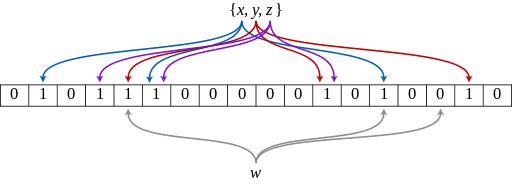
\includegraphics[width=\linewidth]{figures/Bloom_filter.png}
    \caption{An example of a Bloom filter, representing the set $\{x, y, z\}$. The coloured arrows show the positions in the bit array that each set element is mapped to. The element $w$ is not in the set $\{x, y, z\}$, because it hashes to one bit-array position containing 0. For this figure, the bit array has a length of 18 and 3 hash functions are used.\protect\footnotemark}
    \label{fig:bloom_filter}
\end{figure}

\footnotetext{
    Figure from \url{https://commons.wikimedia.org/wiki/File:Bloom_filter.svg} and caption adapted from \url{https://en.wikipedia.org/wiki/Bloom_filter\#/media/File:Bloom_filter.svg}.
}

The authors propose a novel method of applying the Bloom filter to language modelling. They first quantise the language model statistics (the frequency count of a given n-gram) using a logarithmic codebook:
$$ qc(x) = 1 + \lfloor log_b c(x) \rfloor $$
where $qc(x)$ is the quantised frequency count of a given n-gram $x$, $_b$ is the base of the logarithm that controls the granularity of the quantisation, and $c(x)$ is the frequency count of $x$. Each n-gram is then hashed by itself with its quantised frequency count appended to it. However, due to the nature of the Bloom filter, using it to store the exact quantised frequency is liable to errors. The authors take advantage of the one-sided error and hash each n-gram appended with the numbers one through to $qc(x)$. For example, if the bigram ``Computer Science'' has a quantised frequency of three, then the entries ``Computer Science1'', ``Computer Science2'', ``Computer Science3'' will be hashed into the Bloom filter. When retrieving the quantised frequency for the bigram, the bigram is suffixed with the numbers one through $N$, where $N$ is the maximum quantised frequency, stopping at the first occurrence of zero. In the case of the example, we would get zero at ``Computer Science4'' meaning the quantised frequency for the bigram is at most three. As we can see this method gives a upper bound on the quantised frequency for a given n-gram, sacrificing precision.

Putting all of this together, Talbot and Osborne construct a simple yet memory efficient n-gram language model based on the Bloom filter. However, due to the construction of the Bloom filter it is possible that false positives occur. The authors approach this problem by leveraging the one-sided error property of the filter and opt for giving the upper bound for the quantised frequency of a n-gram. Their method is also configurable such that it can be optimised for higher precision and lower error rate, or lower memory usage according to what is needed. One thing the authors do not go into is how fast their method is.

\section{A Succinct N-gram Language Model} 
In 2009 Watanabe et al. \cite{watanabe2009succinct} investigated ways of further improving the memory efficiency of the LOUDS tree structure representation \cite{jacobson1989space, rahman2006engineering}.
Their main contributions are:
\begin{itemize}
    \item modifications to the original LOUDS method that reduces its memory usage
    \item experiments showing how much further memory can be saved by using variable-length coding and block-wise compression (\verb|zlib| as used in GNU \verb|gzip|) on the data.
\end{itemize}

\begin{figure}
    \centering
    
    \begin{subfigure}{0.7\linewidth}
         \centering
         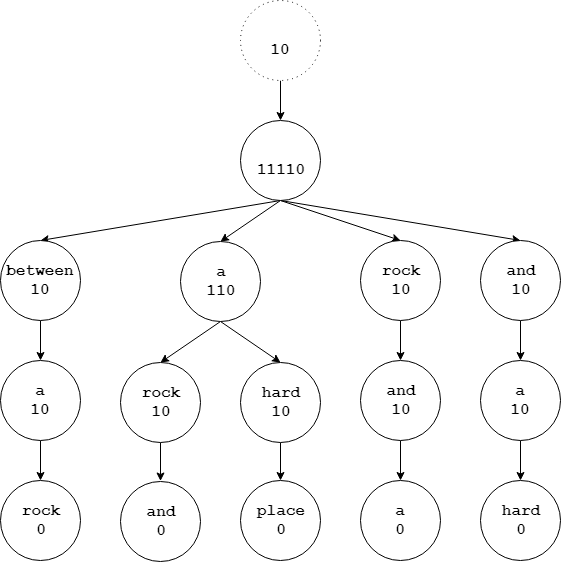
\includegraphics[width=\textwidth]{figures/LOUDS.png}
         \caption{Trie Data Structure}
         \label{fig:louds_trie}
     \end{subfigure}
     
     \begin{subfigure}{\linewidth}
         \centering
         \begin{tabular}{|c?c?c|c|c|c?c|c|c|c|c?}
            \hline
            10 & 11110 & 10 & 110 & 10 & 10 & 10 & 10 & 10 & 10 & 10 \\
            \hline
         \end{tabular}
         
         \begin{tabular}{c|c|c|c|c|}
            \hline
            0 & 0 & 0 & 0 & 0 \\
            \hline
         \end{tabular}
         
         \caption{LOUDS Bit String}
         \label{fig:louds_bit_string}
     \end{subfigure}
     
     \begin{subfigure}{\linewidth}
         \centering
         \begin{tabular}{|c|c|c|c?c|c|c|c|c|}
            \hline
            10 & 110 & 10 & 10 & 10 & 10 & 10 & 10 & 10 \\
            \hline
         \end{tabular}
         
         \caption{Watanabe et al. LOUDS Bit String}
         \label{fig:watanabe_louds_bit_string}
     \end{subfigure}

    \caption{An example of using a trie for representing a n-gram collection (top), the corresponding LOUDS bit string representation of the tree structure (middle), and an example of the optimised version of the LOUDS bit string that Watanabe et al. propose (bottom). Figure \ref{fig:louds_trie} illustrates a trie consisting of trigrams generated from the phrase ``between a rock and a hard place''. The node with the dotted outline is the \textit{super-root} node. Written in each node is the word it represents and its degree in unary.
    Figure \ref{fig:louds_bit_string} shows the resulting LOUDS bit string broken up over two lines. The thick lines show where the levels of the trie stop and start.
    }
    \label{fig:louds_example}
\end{figure}

Level-order unary degree sequence (LOUDS) is a compact representation that uses a $2M + 1$ bit string to represent a tree structure with $M$ nodes. Rather than using explicit pointers which can use up quite a bit of space in large data structures, it uses this bit string for traversal of the tree structure. It is constructed by traversing the tree in breadth-first order. The degree of each node (i.e. the number of child nodes) is encoded as a unary bit string and appended to the bit string. The original author adds a \textit{super-root} node in order to maintain the ``one \textbf{1} per node'' property \cite{jacobson1989space}. An example is shown in Figure \ref{fig:louds_example}.
%As shown in Figure \ref{fig:louds_example}, there is exactly one \textbf{1} and one \textbf{0} for each node plus one extra \textbf{0}, leading to a 23-bit bit string for tree where $M=11$ - which is exactly $2M + 1$.

Two optimisations that the authors apply to the LOUDS representation are removing the bits representing the root node and the leaf nodes. These are unnecessary if the starting position of the bigrams and the highest order n-grams (i.e. the leaf nodes in the trie) are recorded as integers instead. Using these optimisations we can save a number of bits equal to the number of unigrams and highest order n-grams in the dataset. However, these optimisations have little effect in the grand scheme of things. They report their results on the Web 1T 5-gram dataset which is about 24GB when compressed with gzip. In the dataset there about 13.5 million unigrams and 1.1 billion 5-grams. Thus, in this case Watanabe et al. save about 13.5 million bits (about 1.7MB) by omitting the root node from the LOUDS bit string, and about 1.1 billion \texttt{0} bits (about 138MB) by omitting the highest order n-grams. However, even their most compact representation of the Web 1T 5-gram dataset is about 9.8GB, so the advantage gained by these optimisations is only about 1\%. So assuming that these approximate calculations are correct, it would seem that these optimisations have very little effect, and are unnecessary unless you really need to save those few hundred megabytes of memory.

Watanabe et al. decrease the memory usage of the word IDs and counts by applying a variable length encoding and block-wise compression. The variable length encoding that they introduce is almost identical to variable byte encoding. The only difference is instead of storing the bit indicating when an integer has ended within the byte sequence, they store these bits in a separate bit string. With this integer encoding they are able to save about 6GB (or about 9.2\%) over the method proposed in \cite{raj2003lossless} which they use as one of the baselines. They further compress the data by compressing it in 8KB blocks using \texttt{zlib} and facilitate random access by recording the compressed blocks' starting offsets. With this they are able to reduce the total memory usage by about 33\%.

Compared to the work of Talbot and Osborne, the advantage of the work of Watanabe et al. is that their compression is lossless and yet it provides a comparable compression rate. However, Watanabe et al. do not run experiments evaluating the speed of their methods and interestingly enough they simply conclude that their representation of the n-grams is ``practical enough''. 

Fortunately, the authors of \cite{pibiri2019handling} perform extensive experiments to evaluate the performance of various n-gram representations, including this one. In these experiments the authors use the publicly available code of Watanabe et al., and Talbot and Osborne's work (henceforth referred to as Expgram and RandLM respectively). On the Europarl dataset\footnote{\url{http://www.statmt.org/europarl}} Expgram uses about 13.8\% more memory than RandLM (about 2.06 bytes per n-gram for Expgram) however on average it was about 36.2\% faster than RandLM (2.8 $\mu$sec/query for Expgram). Interestingly, Expgram does not scale well and when tested on the YahooV2 dataset\footnote{\url{http://webscope.sandbox.yahoo.com/catalog.php?datatype=l}} it loses its speed advantage and ends up about 81.6\% percent slower (9.23 $\mu$sec/query for Expgram). Furthmore, the authors of \cite{pibiri2019handling} could not get Expgram to work on the GoogleV2 dataset\footnote{\url{http://storage.googleapis.com/books/ngrams/books/datasetsv2.html}}, whereas RandLM worked fine.

So while the work of Watanabe et al. in their 2007 paper looks promising and provides better performance than Talbot and Osborne's work on smaller datasets, it struggles to scale well with larger scale datasets such as the YahooV2 and GoogleV2 datasets.

% \section{Faster and smaller n-gram language models}
% In 2011 Pauls and Klein \cite{pauls2011faster} explore a few different variations on the trie data structure and try formulate a method that is both faster and smaller than a popular language modelling toolkit - SRILM. 
% Their main contributions are:
% \begin{itemize}
%     \item a trie representation of n-grams that is as fast as SRILM but uses 25\% less memory
%     \item a novel method for speeding up queries in machine translation tasks by exploiting patterns in the queries
% \end{itemize}


% Pauls and Klein explore three different 

% Much like the work of Watanabe et al. they explore the use of variable length coding. They also show that the last word of each n-gram can be implicitly encoded, and they make use of a block-based compression scheme. They also observe patterns in the queries to the language models and exploit these observations. They discover that within their experimental setup only one million out of the 31 million queries are unique. To exploit this they add a simple cache to speed up repeated queries.
% They also observe that it is often the cast that the last $n - 1$ tokens of a n-gram query constitute the first $n - 1$ the following query. As such, the authors devise a scheme for encoding the context (the $n - 1$ trailing tokens in a n-gram) and using that for the next query.

% They report that their hash-table based method outperforms SRILM (a popular fast language model toolkit) in both terms of time and space. However, their claim is a bit shaky since they introduce a handicap to the SRILM implementation by calling it via the Java Native Interface (SRILM is implemented in C++). The authors imply that without this added overhead SRILM would be about twice as fast. What they do not say is that without this overhead SRILM would then be faster than all of their implementations. Nonetheless, their proposed methods are indeed fast and small as shown in the experiments in \cite{pibiri2019handling}.

\section{Handling Massive N-Gram Datasets Efficiently} \label{sec:new_state_of_the_art}
This paper \cite{pibiri2019handling} was recently published in the 2019 ACM Transactions on Information Systems (TOIS). Pibiri and Venturini explore methods of improving n-gram representations to produce a method that is compact, fast and lossless. Their main contributions are:
\begin{itemize}
    \item a compressed trie data structure in which each level of the trie is modelled as a
monotonic non-decreasing integer sequence that is encoded with Elias-Fano which allows constant time access
    \item a method for further decreasing the memory usage of the trie data structure by reducing the magnitude of the integers that represent the trie's structure.
    \item an improvement over the state of the art implementation of Kneser-Ney smoothing that reduces I/O and increases performance more than two-fold.
\end{itemize}

Their main result is the Elias-Fano trie. This formulation is similar to that of LOUDS in the way logical pointers are used instead of physical pointers in order to save space. Whereas LOUDS uses a unary bit string to represent the tree structure, the trie structure proposed by Pibiri and Venturini uses Elias-Fano encoded \cite{elias1974efficient, fano1971number} integer sequences. The main advantage of the Elias-Fano encoding is that it allows constant time random access without costly decoding. This encoding scheme relies on the integer sequence being monotonic non-decreasing, so the authors transform the word IDs in each level of the trie to satisfy this constraint. One disadvantage of the Elias-Fano encoding is that does not take advantage of sequences of integers that are all close together (i.e. have small deltas) -- something that occurs often in data structures such as inverted indexes. There is a variant of the Elias-Fano encoding called partitioned Elias-Fano encoding that can take advantage of this property \cite{ottaviano2014partitioned}. In this variant the integer sequence is partitioned into chunks. The representation is further split into two levels: the first level contains the last element of each chunk and the second level contains the encoding of the chunks themselves. Essentially, the partitioned Elias-Fano encoding sacrifices a bit of speed for a more compact representation.

In Pibiri and Venturini's trie each level is represented as a set of three arrays: an array of word IDs, an array of pointers (integer offsets) indicating where the successor/child nodes of a given node start and finish in the next level, and an array of frequency counts. By construction the pointer array is sorted and immediately Elias-Fano encodable, however the word ID array is not. If we consider the set of unigrams \{A, B, C, D\} and the set of bigrams \{AA, AC, BB, BC, BD, CA, CD, DB, DD\} from the example in Figure \ref{fig:elias_fano_trie}, and given that the unigrams have the word IDs \{0, 1, 2, 3\}, the word ID array of the second level would look like this: \texttt{\{0, 2, 1, 2, 3, 0, 3, 1, 3\}}. As we can see this is not monotonically non-decreasing as the Elias-Fano encoding requires. The authors solve this problem by transforming the word IDs with a range-wise prefix sum. Initially this sum is set to zero. Then for each node in the level we add the prefix sum to the word IDs of the nodes that have the same parent (i.e. are sibling nodes) and then update the prefix sum to be equal to the maximum word ID of the sibling nodes. In the above example the first set of nodes have the word IDs \{0, 2\}, since the initial prefix sum is zero there is no change to the word IDs and the prefix sum is set to the word ID of the right-most sibling. The next set of sibling nodes is \{1, 2, 3\} so we add 2 to each word ID giving the new word IDs \{3, 4, 5\} and we update the prefix sum to 5 and repeat this for the rest of the nodes in the level. This results in the word ID sequence \texttt{\{0, 2, 3, 4, 5, 5, 8, 9, 11\}} as shown in the example in Figure \ref{fig:elias_fano_trie}. With this the authors are able to apply Elias-Fano encoding to the word ID and pointer arrays, allowing them to represent the trie structure compactly whilst still allowing for contstant time random access.

\begin{figure}
    \centering
    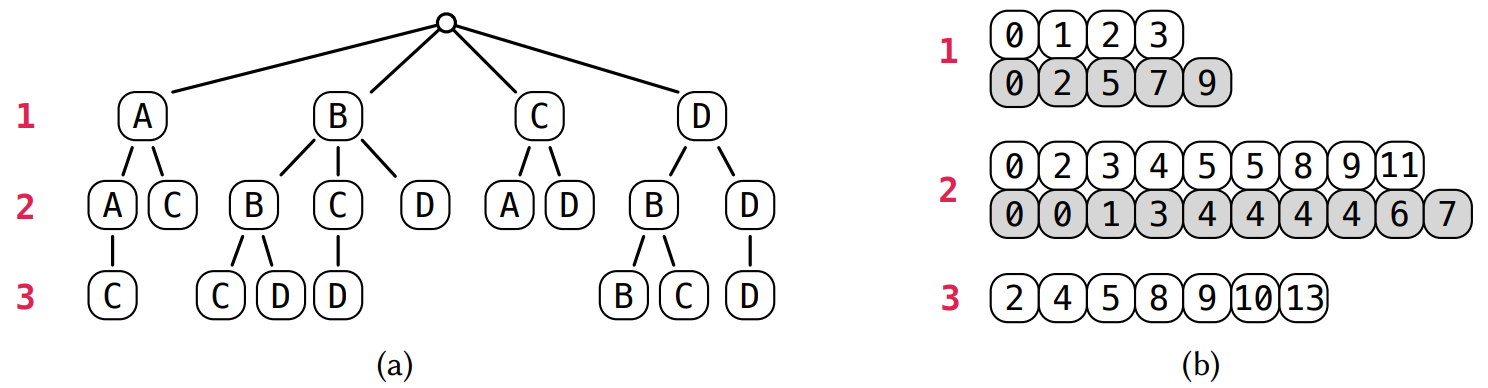
\includegraphics[width=\linewidth]{figures/elias-fano_trie.png}
    \caption{On the left (a): example of a trie of order 3, representing the set of grams \{A, AA, AAC, AC, B, BB, BBC, BBD, BC, BCD, BD, CA, CD, DB, DBB, DBC, DDD\}. On the right (b): the sorted-array representation of the Elias-Fano trie. Light-grey arrays represent the word IDs transformed into monotonic sequences using range-wise prefix sums and the dark-grey arrays represent the position in the next level where the successors of each node start and finish.\protect\footnotemark}
    \label{fig:elias_fano_trie}
\end{figure}

\footnotetext{Figure and caption adapted from the paper \cite{pibiri2019handling}.}

Another important optimisation that Pibiri and Venturini add is array-rank encoding of the frequency counts. This method takes advantage of certain properties of n-gram collections. One such property is that the distribution of frequency counts is Zipfian, there are a few n-grams that appear frequently and the rest (i.e. the majority) only appear occasionally. Another property is that if we look at the unique frequency counts we notice that the number of these is much smaller than the range of the frequency counts. These properties can be taken advantage of to reduce the space requirements. First, we store the unique frequency counts in an array meaning less frequency counts need to be stored. As mentioned before, each level of the trie uses three arrays, one of which stores the frequency counts. Rather than storing the frequency counts directly, which could be inefficient in space due to the possible large range of frequency counts requiring a large number of bits per frequency count, we instead store the corresponding rank of the frequency count in the array of unique frequency counts. These sequences of rank values are not monotonic non-decreasing so they cannot be Elias-Fano encoded, however the values are highly repetitive so instead they are coded with a binary codebook such that frequency counts that occur often are assigned shorter codes. With this optimisation the authors are able further reduce the space requirements of the n-gram language model.

Overall we can see that the optimisations implemented by Pibiri and Venturini leads to a n-gram representation that is both compact and fast, while remaining lossless. They use a few other tricks to further improve their n-gram representation but I will not go into these due to space restrictions. Their method is also competitive with previous state-of-the-art methods, including Talbot and Osborne's and Watanabe et al's work, in both space and time. Pibiri and Venturini's extensive experimental analysis shows that their PEF (partioned Elias-Fano) trie is more compact and faster than a collection of the recent state-of-the-art methods \cite{talbot2007randomised, watanabe2009succinct, pauls2011faster}, and even more compact than the lossy method introduced by Talbot and Osborne. While PEF trie is still slower than the fastest hash table based method they tested (by about 1.5$\mu$sec/query or 81.5\% slower), PEF trie was close to $4\times$ more space efficient than the most compact hash table based method tested. Another advantage that PEF trie has over current methods is that it scales better and gains more of an advantage in both space and time efficiency over the other methods as the dataset gets larger. Also, many of the tested methods failed to run on the GoogleV2 dataset. So if you need to use large n-gram datasets then it seems like Pibiri and Venturini's PEF trie is the way to go. 

\section{Future Work}
% Query throughput is important especially when a large volume of queries need to be served at any given moment. At 1.73 $\mu$sec/query on the YahooV2 dataset PEF trie was about 34.4\% slower than the slowest hash table based method and 81.5\% slower (about $5\times$ slower) than the fastest hash table based method the authors tested. It would be interesting to see how the trade-off between space and time plays out between PEF trie and these hash table based methods. Clearly for using large n-gram datasets on a single machine PEF trie is the obvious choice due to the lower space requirements, however the hash table based methods could have their space requirements spread across multiple machines in a massively distributed system. Doing some rough calculations the PEF trie should be able to serve about 578,000 queries per second, whereas the minimal perfect hash (MPH) method they test against should be able to serve about 3,125,000 queries per second. If we assume the entire storage needed to store an arbitrary n-gram dataset with PEF trie was about 32GB and we were using a machines with about that much RAM, the MPH method would need distributed across about three machines in order to store the entire dataset once. However, to reach the same throughput as the MPH method you would need about 5-6 of these machines running PEF trie. Of course this is bit of a contrived and oversimplified example, but I think it illustrates that if maximising query throughput is the primary concern then hash table based methods are probably best. So it would be interesting to see how this plays out in reality.

Query throughput is important especially when a large volume of queries need to be served at any given moment. It would be interesting to see how the time-space trade-off would play out between PEF trie and the hash table based methods. The hash table based methods require many times more memory but are up to many times faster than PEF trie. To store the same amount of data the hash table based methods would require many times more RAM but would offer a higher query throughput. Conversely, PEF trie would require many times less RAM but in order to offer equivalent query throughput would require multiple instances of PEF trie to be run in parallel. So it would be interesting to investigate the cost of these two approaches in terms of the hardware required to provide equivalent query throughput.

The papers discussed in this review apply existing methods in interesting ways or introduce novel methods that give impressive results in creating efficient n-gram language models. It would be interesting to see if the lessons learned from these papers could be, or have already been, applied to other tasks.

\section{Conclusion}
In this review we have covered three papers that take different approaches to creating efficient n-gram representations. Talbot and Osborne apply Bloom filters to language modelling and devise a compact representation that trades off space and precision. Watanabe et al. propose improvements to the LOUDS tree representation and demonstrate the effectiveness of LOUDS in conjunction with variable-length integer encoding. Finally, Pibiri and Venturini apply optimisations to the trie-based n-gram language model representation that allows for extensive use of Elias-Fano encoding. They further close the gap between hash-based and non hash-based methods in terms of speed while providing one the most compact n-gram representations to date.

%
% The next two lines define the bibliography style to be used, and the bibliography file.
\bibliographystyle{ACM-Reference-Format}
\bibliography{report}

\end{document}
